\documentclass[../Head/Main.tex]{subfiles}
\begin{document}

\subsection{Effectiveness of lidar marble detection}

The purpose of this test is establish the effectiveness of the marble detection algorithm for the lidar sensor.

\subsubsection*{Description of test}
The initial position of the robot for this test is the origin of the environment \texttt{bigworld}. Here the robot is steered around in the environment using the keypad. The idea of this test is to test if all marbles detected by the algorithm actually corresponds to marbles in the environment.     

\subsubsection*{Test parameters}
\begin{tabular}{l r}
	- World used                & bigworld\\	
	- Number of spawn marbles   & 20\\
	- Number of tests           & 9\\
	- Range between two points  & 0.2\\
	- Range to marbles in outer edges of sensor range & 9.8
\end{tabular}

\subsubsection*{Data}
\begin{figure}[H]
  \begin{subfigure}[b]{0.3\textwidth}
  	\centering
    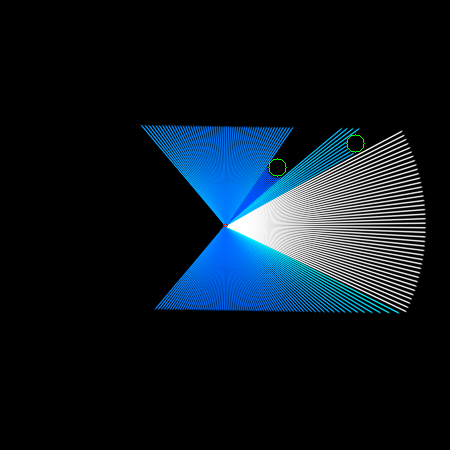
\includegraphics[width=1\textwidth]{Lidar/Test_1_marbles}
    \caption{Illustration of data for test 1}
    \label{fig:Marbletest1}
  \end{subfigure}
  \hfill
  \begin{subfigure}[b]{0.3\textwidth}
  	\centering
    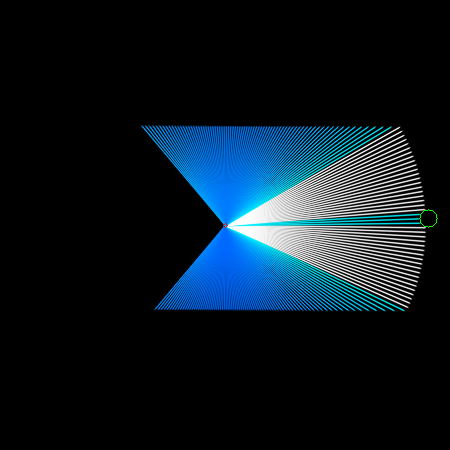
\includegraphics[width=1\textwidth]{Lidar/Test_2_marbles}
    \caption{Illustration of data for test 2}
    \label{fig:Marblestest2}
  \end{subfigure}
  \hfill
  \begin{subfigure}[b]{0.3\textwidth}
    \centering
    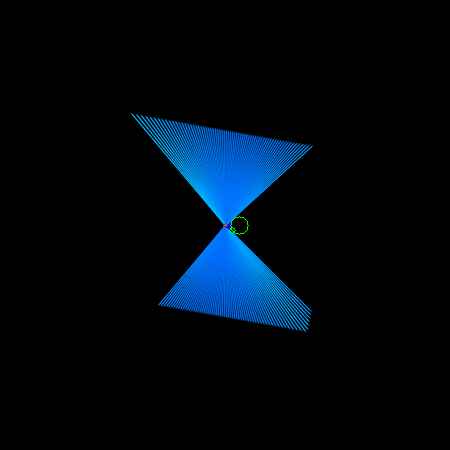
\includegraphics[width=1\textwidth]{Lidar/Test_3_marbles}
    \caption{Illustration of data for test 3}
    \label{fig:Marblestest3}
  \end{subfigure}
  \hfill
  \begin{subfigure}[b]{0.3\textwidth}
    \centering
    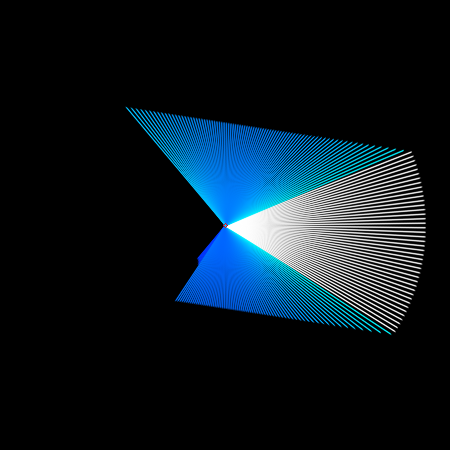
\includegraphics[width=1\textwidth]{Lidar/Test_4_marbles}
    \caption{Illustration of data for test 4}
    \label{fig:Marblestest4}
  \end{subfigure}
  \hfill
  \begin{subfigure}[b]{0.3\textwidth}
    \centering
    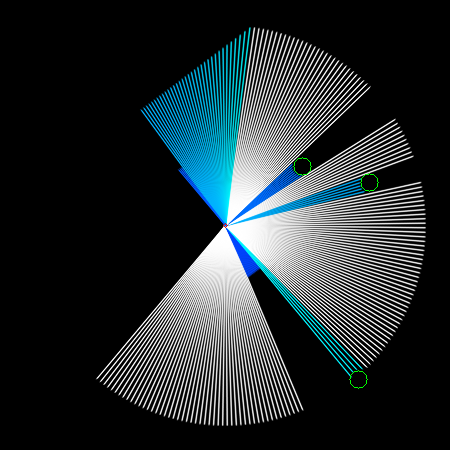
\includegraphics[width=1\textwidth]{Lidar/Test_5_marbles}
    \caption{Illustration of data for test 5}
    \label{fig:Marblestest5}
  \end{subfigure}
  \hfill
  \begin{subfigure}[b]{0.3\textwidth}
    \centering
    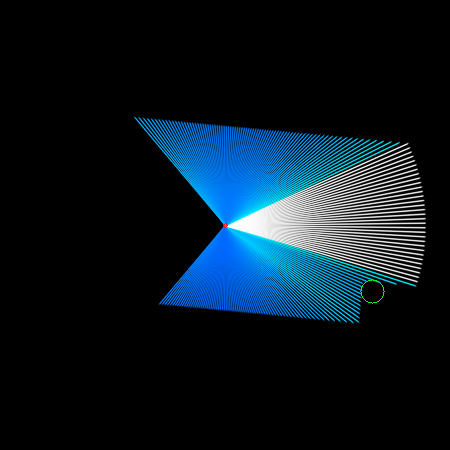
\includegraphics[width=1\textwidth]{Lidar/Test_6_marbles}
    \caption{Illustration of data for test 6}
    \label{fig:Marblestest6}
  \end{subfigure}
  \caption{Illustration of data for marble detection test 1-6}
  \label{fig:Marblestests16}
\end{figure}
\begin{figure}[H]
  \begin{subfigure}[b]{0.3\textwidth}
    \centering
    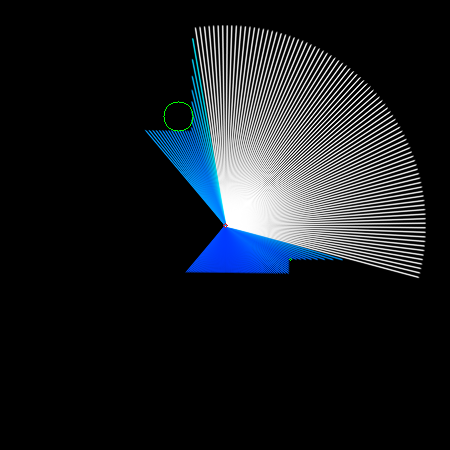
\includegraphics[width=1\textwidth]{Lidar/Test_7_marbles}
    \caption{Illustration of data for test 7}
    \label{fig:Marblestest7}
  \end{subfigure}
  \hfill
  \begin{subfigure}[b]{0.3\textwidth}
    \centering
    
\includegraphics[width=1\textwidth]{Lidar/Test_8_marbles}
    \caption{Illustration of data for test 8}
    \label{fig:Marblestest8}
  \end{subfigure}
  \hfill
  \begin{subfigure}[b]{0.3\textwidth}
    \centering
    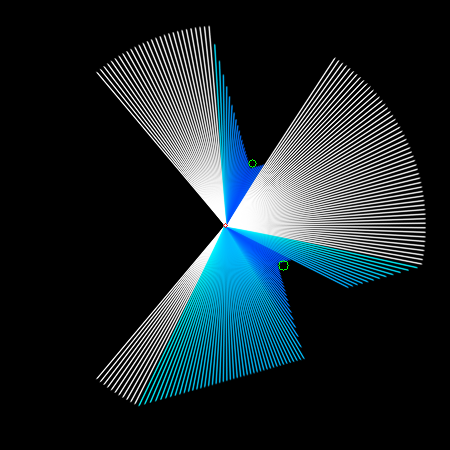
\includegraphics[width=1\textwidth]{Lidar/Test_9_marbles}
    \caption{Illustration of data for test 9}
    \label{fig:Marblestest9}
  \end{subfigure}
  \caption{Illustration of data for marble detection test 7-9}
  \label{fig:Marblestests79}
\end{figure}

\subsubsection*{Conclusion}
It can be concluded that the marble detection algorithm is not reliable, since it in some cases detects more than one marble, marbles in corners and marbles of different size.
\end{document}